\section{Deep learning}

\begin{itemize}
		\item Machine learning: Decisions determined by a model trained on data
		\item Deep learning: Machine learning based on neural networks
		\item Historically not applicable because of vanishing gradient problem
				(slow convergence), but recent progress due to better
				algorithms, increased processing power and large datasets
\end{itemize}

\subsection{Perceptron}

\begin{itemize}
		\item Calculates weighted sum of inputs
		\item Bias to shift value
		\item Non-linear activation function determines whether output activates or not
\end{itemize}

\[
		\hat{y} = g (w_0 + \sum_{i = 1}^m x_i w_i)
\]

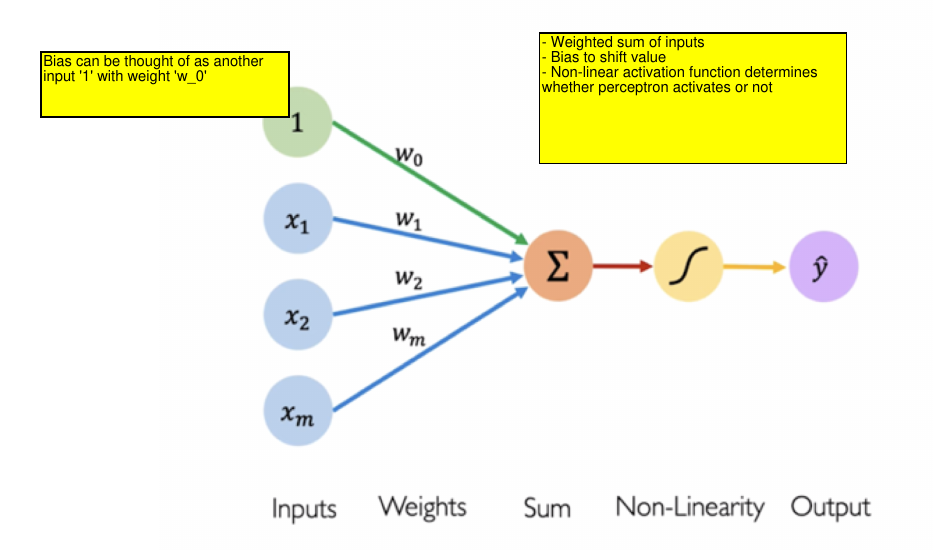
\includegraphics[width=0.7\textwidth]{08_perceptron}

\subsubsection{Common activation functions}

\paragraph{Sigmoid function}

\begin{align*}
		g(z) & = \frac{1}{1 + e^{-z}} \\
		g'(z) & = g(z) \cdot (1 - g(z))
\end{align*}

\paragraph{Hyperbolic tangent}

\begin{align*}
		g(z) & = \frac{e^z - e^{-z}}{e^z + e^{-z}} \\
		g'(z) & = 1 - g(z)^2
\end{align*}

\paragraph{Rectified linear unit}

\begin{align*}
		g(z) & = \max(0, z) \\
		g'(z) & = \left\{\begin{array}{lr}
						1, & \text{for } z > 0 \\
						0, & \text{otherwise} \\
		\end{array}\right.
\end{align*}

\subsection{Single layer neural network}

\begin{itemize}
		\item One hidden layer of perceptrons
		\item Fully connected
		\item One weight matrix per perceptron (with one weight per input each) for input -> hidden transition
		\item And one weight matrix per perceptron for hidden -> output transition
		\item Final outputs are then weighted sums of each perceptron's output,
				again with a weight per perceptron / final output pair, fed
				once more through non-linear activation function.
				\begin{itemize}
						\item Final outputs are effectively perceptrons too,
								which use hidden layer as inputs.
				\end{itemize}
\end{itemize}

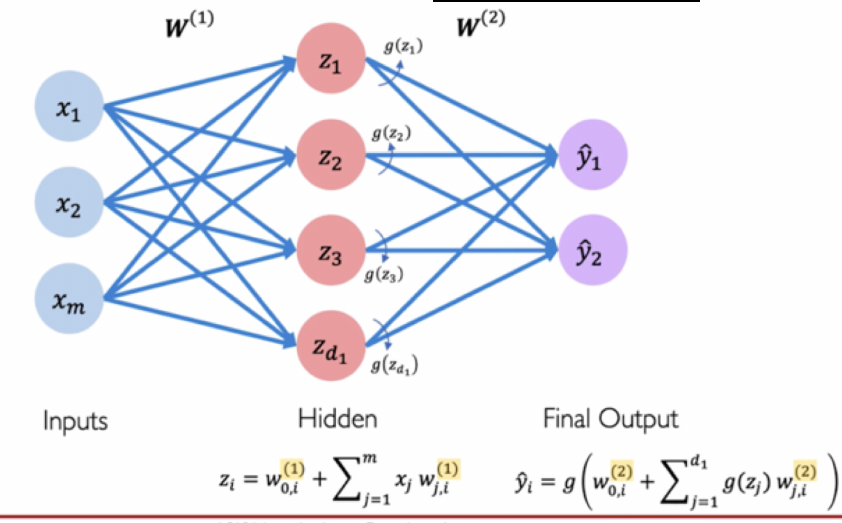
\includegraphics[width=0.7\textwidth]{08_single_layer}

\subsection{Deep neural network}

\begin{itemize}
		\item Many (in practice: several hundred) hidden layers, each consuming
				outputs of previous layer.
\end{itemize}

\subsection{Empirical loss}

\begin{itemize}
		\item Measures total loss over dataset.
		\item `Cost' incurred to network if predicted output incorrect, used to
				train network by making it minimize loss.
		\item During training, network finds weights such as to minimize loss.
\end{itemize}

\begin{align*}
		J(W) = \frac{1}{n} \sum_{i = 1}^n L(f(x^{(i)}; W), y^{(i)})
\end{align*}

Where $x$ inputs, $y$ labels, $f(x)$ predictions, $W = \{W^{(i)}$ weights,
		$J(W)$ total loss, $L()$ loss function, $f(x^{(i)}; W)$ predicted given
		set of weights.

\subsection{Loss optimization}

Find weights $W*$ which achieve lowest loss:

\begin{align*}
		W* = \operatorname{argmin}_W J(W)
\end{align*}

\subsection{Gradient descent}

Move along `down' direction in multidimensional space until convergence.

\subsubsection{Backpropagation}

Problem: How to figure out how to change weights to go `down'? Idea: Use chain
rule to recursively figure out effect changes to weight will have on loss.

Example: Shows how changes to $w_1$ will affect final loss.

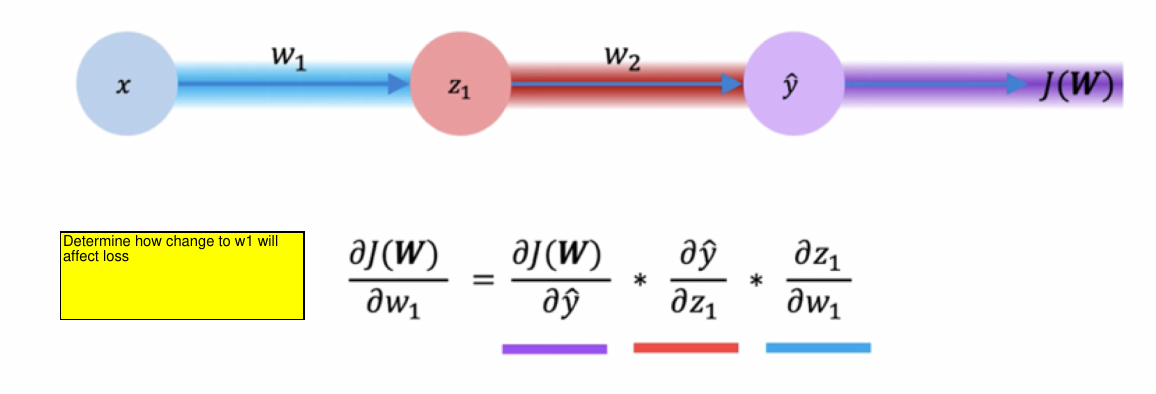
\includegraphics[width=0.7\textwidth]{08_backpropagation}

\subsubsection{Gradient descent algorithm}

\begin{enumerate}
		\item Initialize weights randomly with normal distribution around $0$
		\item Loop until convergence:
				\begin{enumerate}
						\item Compue gradient $\frac{\partial J(W)}{\partial W}$
						\item Update weights $W \coloneqq W - \eta
								\frac{\partial J(W)}{\partial W}$ with learning
								rate $\eta$
				\end{enumerate}
		\item Return weights
\end{enumerate}

\subsubsection{Stochastic gradient descent}

To accelerate convergence: Instead of calculating gradient over full dataset
(costly), use random batch $B$ (order 10s - 100s) over which to calculate
gradient:

\begin{align*}
		\frac{\partial J(W)}{\partial W} = \frac{1}{B} \sum_{k = 1}^B \frac{\partial J_k(W)}{\partial W}
\end{align*}

\subsubsection{Avoiding local minima}

\begin{itemize}
		\item Repeat training with multiple initializations
		\item Adapt learning rates. Too low has risk of being stuck in local
				minima, too high has risk of overshooting.
		\item Less risk of local minima in higher-dimensional spaces.
\end{itemize}

\subsection{Avoiding over-fitting}

\begin{itemize}
		\item Dropout: Randomly set certain weights per layer to 0, prevent
				network from becoming too complex
		\item Early stopping: Separate validation set, stop training once
				validation set minimized loss
\end{itemize}
